\documentclass[conference]{IEEEtran}
\IEEEoverridecommandlockouts
% The preceding line is only needed to identify funding in the first footnote. If that is unneeded, please comment it out.
\usepackage{cite}
\usepackage{amsmath,amssymb,amsfonts}
\usepackage{algorithmic}
\usepackage{graphicx}
\usepackage{textcomp}
\usepackage{xcolor}
\usepackage{booktabs}
\usepackage{url}
\def\BibTeX{{\rm B\kern-.05em{\sc i\kern-.025em b}\kern-.08em
    T\kern-.1667em\lower.7ex\hbox{E}\kern-.125emX}}
\begin{document}

\title{Data Mining Project: Analyzing Reader Patterns and Genre Associations in the Goodreads Dataset*\\
{\footnotesize \textsuperscript{*} CS 4412: Data Mining}
\thanks{Identify applicable funding agency here. If none, delete this.}
}

\author{\IEEEauthorblockN{1\textsuperscript{st} David Holland}
\IEEEauthorblockA{\textit{Student at Kennesaw State University} \\
Marietta GA \\
dholla36@students.kennesaw.edu}

}

\maketitle

\begin{abstract}
This proposal outlines a data mining project focused on the 2017 Goodreads dataset. This study aims to discover relationships between book genres, user behaviors, and how readers structure their reviews. We will be applying different techniques such as Association Rule Mining, K-Means Clustering, and Latent Dirichlet Allocation. This proposal seeks to understand how readers associate different genres in an attempt to define different segments of the reading community.
\end{abstract}

\begin{IEEEkeywords}
Data Mining, Goodreads, Association Rules, Clustering, Text Mining, Pattern Discovery
\end{IEEEkeywords}

\section{Introduction}
The digital age has transformed reading from a personal, solo activity into a social activity. Various platforms like Goodreads and Fable provide a massive database of user-generated data through ratings, reviews, and custom shelves. While many similar projects exist to predict user's rating there is more value in understanding how users engage with literature. This project focuses on the UCSD Goodreads dataset to find these patterns.

\section{Description}
This project will utilize the Goodreads Book Datasets (2017) curated by Julian McAuley at UCSD, Rishabh Misra and Ndapap Nakashole

\subsection{A. Source and Scale }
\begin{itemize}
    \item \textbf{Source:} \url{https://cseweb.ucsd.edu/~jmcauley/datasets/goodreads.html}
    \item \textbf{Size:} The full dataset contains metadata for 2.36 million books and 15.7 million detailed review texts. For this project, a subset (e.g., the "Young Adult" or "History" category) will be utilized to maintain computational feasibility while ensuring a sample size of over 100,000 records.
    \item \textbf{Format:} Data is provided in the CSV and json format, requiring significant preprocessing and flattening.
\end{itemize}

\subsection{Key Features and Schema}
The dataset is split into two primary components:
\begin{enumerate}
    \item \textbf{Metadata (\textit{goodreads\_books.json}):} Contains \texttt{book\_id}, \texttt{title}, \texttt{authors}, \texttt{average\_rating}, and importantly, \texttt{popular\_shelves} (user-defined tags).

    \item \textbf{Reviews (\textit{goodreads\_reviews.json}):} Contains \texttt{user\_id}, \texttt{book\_id}, \texttt{rating}, \texttt{review\_text}, and \texttt{n\_votes}.
    \item \textbf{User Interactions (\textit{goodreads\_interactions.csv}):} Contains \texttt{user\_id}, \texttt{book\_id}, \texttt{is\_read}, \texttt{rating}, and \texttt{is\_reviewed}.
\end{enumerate}


\section{C. Data Quality and Preprocessing}

Known issues include many user-defined shelves that share common tags like "to-read" and varying review lengths. This is most likely caused from Goodread's ability to easily add books to user's "to-read" shelve. Preprocessing will involve tokenization, stop-word removal for text mining and transforming the nested JSON shelves into a transaction-style for association mining.

\section{Discovery Questions}

This project moves beyond prediction models to investigate the following questions the team had:
\begin{itemize}
    \item What are the hidden associations between specfic book genres and user-defined "shelves"? (Do readers of "Romantasy" (Romance Fantasy) also show high interset in other genres like fantasy?
    \item Can we identify distinct Reader Personas based on interaction metrics? By clustering users based on their average rating variance, review frequency, and review length our goal is to discover if it is possible to classify readers as a critical reviewer or casual consumer.
    \item What type of patterns emerge from highly-voted reviews compared to low-voted ones?
\end{itemize}

\section{Planned Techniques}
The analysis will follow a multistage data mining pipeline as visualized in Figure 1.

\begin{figure}[htbp]
  \centering
  \framebox{\parbox{0.5\textwidth}{\centering
    \vspace{0.5cm}
    \textbf{Analysis Pipeline Diagram} \\
    \vspace{0.5cm}
    \small
    \textbf{1. Data Ingestion:} Books \& Reviews JSON Parsing \\
    $\downarrow$ \\
    \textbf{2. Preprocessing:} Admin Tag Cleaning \& Language Filtering \\
    $\downarrow$ \\
    \textbf{3. Mining Modules \& Evaluation:}\\
    \vspace{0.2cm}
    $\rightarrow$ \textit{Shelf Tags} $\Rightarrow$ \textbf{FP-Growth} $\Rightarrow$ Genre Associations (DQ1) \\
    $\rightarrow$ \textit{User Metrics} $\Rightarrow$ \textbf{K-Means} $\Rightarrow$ Reader Personas (DQ2) \\
    $\rightarrow$ \textit{Review Text} $\Rightarrow$ \textbf{LDA} $\Rightarrow$ Helpfulness Patterns (DQ3) \\
    \vspace{0.5cm}
  }}
  \caption{Planned Data Mining Workflow mapping specific data features to their respective algorithms and discovery questions.}
  \label{fig:pipeline}
\end{figure}

\subsection{Association Rule Mining (FP-Growth)}\label{AA}
    We will treat each user's shelves as a transaction. Using the FP-Growth Algorithm to discover rules with high lift and confidence to identify non-obvious genre relationships. Our goal is to move beyond the standard "Fantasy" label and discover more sub-genre patterns.
\subsection{Clustering (K-Means)}
    To answer the second discovery question, we will apply K-Means clustering on standarized numerical features derived the user dataset. We will be using the "Elbow Method" and "Silhoutette Score" to determine the optimal number of reader segments.
\subsection{Text Mining (LDA - Topic Modeling)}
    Using the Latent Dirichlet Allocation (LDA) algorithm, we will perform topic modeling on the \texttt{review\_text}. This will allow us to discover the primary topics of discussion within different genres without pre-defining what those topics are.

\section {Preliminary Timeline}
The project will proceed according to the following milestones

\begin{table}[htbp]
\caption{Project Milestone Timeline}
\begin{center}
\begin{tabular}{@{}llp{4.5cm}@{}}
\toprule
\textbf{Milestone} & \textbf{Period} & \textbf{Key Activities} \\ \midrule
M2 & Weeks 8 & Applying KDD process and Association Rule Mining \\
M3 & Weeks 11 & Clustering Analyses, Classification Techniques, detecting Anomalies, and Communicating results \\
M4 & Weeks 14 & Text Mining (LDA), Final Report \\ \bottomrule
\end{tabular}
\end{center}
\end{table}
\subsection{Anticipated Challenges}
\begin{itemize}
    \item   Our primary challenge is lack of experience in analyzing data sets.
    \item Another challenge is the volume of data. The Goodreads dataset is comprised of multiple csv and jsons files that is multiple gigabytes compressed. Handling this in local memory will require using pandas chunking or focusing on smaller genre subsets. Text data can also be "noisy" and will require filtering to produce meaningful topics.
    \item Due to Goodreads' global reach our team expects to encounter non-English reviews, books, and shelf titles. Our team will have to strip any non-English text out of the datasets in order to prevent any of our proposed tests from failing.
\end{itemize}

\section{Milestone 2}

This section details the work done for Milestone 2 of this data mining project. This milestone focused on an inital implementation of an exploratory discovery analysis to initally answer one of our three discovery questions. The section begins by explaining the reasoning for preprocessing and cleaning up the noisy dataset. Our team then analyses the most frequent tags of users' bookshelves to gain a first look at how users cateogrize books on the site. This section also covers our findings on discovery question 1 and how we came to our conclusions.  In addition to discovery question 1, we have provided visualzaitons of our findings.


\subsection{Preprocessing and Data Transformation}

In order to transition from the introductory and theoretical discovery questions from the previous sections our team implemented multiple scripts to select and gather the raw data from the dataset.
 To begin answersing our discovery questions we will need to preprocess our data through a python code to filter the massive dataset by cleaning some administrative tags and filtering out non-English languages. First we performed a keyword search across the "popular\_shelves" attribute of the \texttt{goodreads\_books.json.gz} file. We specifically search for genres: 'romantasy', 'romantic-fantasy', 'fantasy-romance', 'romance', 'fantasy', and 'romantic'. The filtered results are stored in \texttt{01\_filteredbooks.json}. The resulting json consists of records: book\_id, title, average\_rating, shelves\_list.


To answer discovery question 1, we need to examine the different user interactions, so we implemented a second filtering script utilizing the book\_id from our previous script to extract reviews from the \texttt{goodreads\_reviews\_dedup.json.gz} dataset, storing the output in \texttt{03\_extractedreviews.csv}.

The datasets required significant cleaning before our team could conduct meaningful mining. First, we removed generic administrative tags like \texttt{`to-read'} and \texttt{`ebooks'} from the books dataset to reduce noise. Second, to focus our analysis and ensure data comprehension, we removed any non-English records from the reviews dataset using the Python package \texttt{langid}.

\subsection{Exploratory Data Analysis}
Before applying our mining algorithms, our team examined the distributions of ratings, community-defined tags (for example users can create virtual bookshelves and give them a name), and review engagement to establish a baseline understanding of the ``Romantasy'' and other romance genres subset.

 \begin{figure}[htbp]
    \centering
    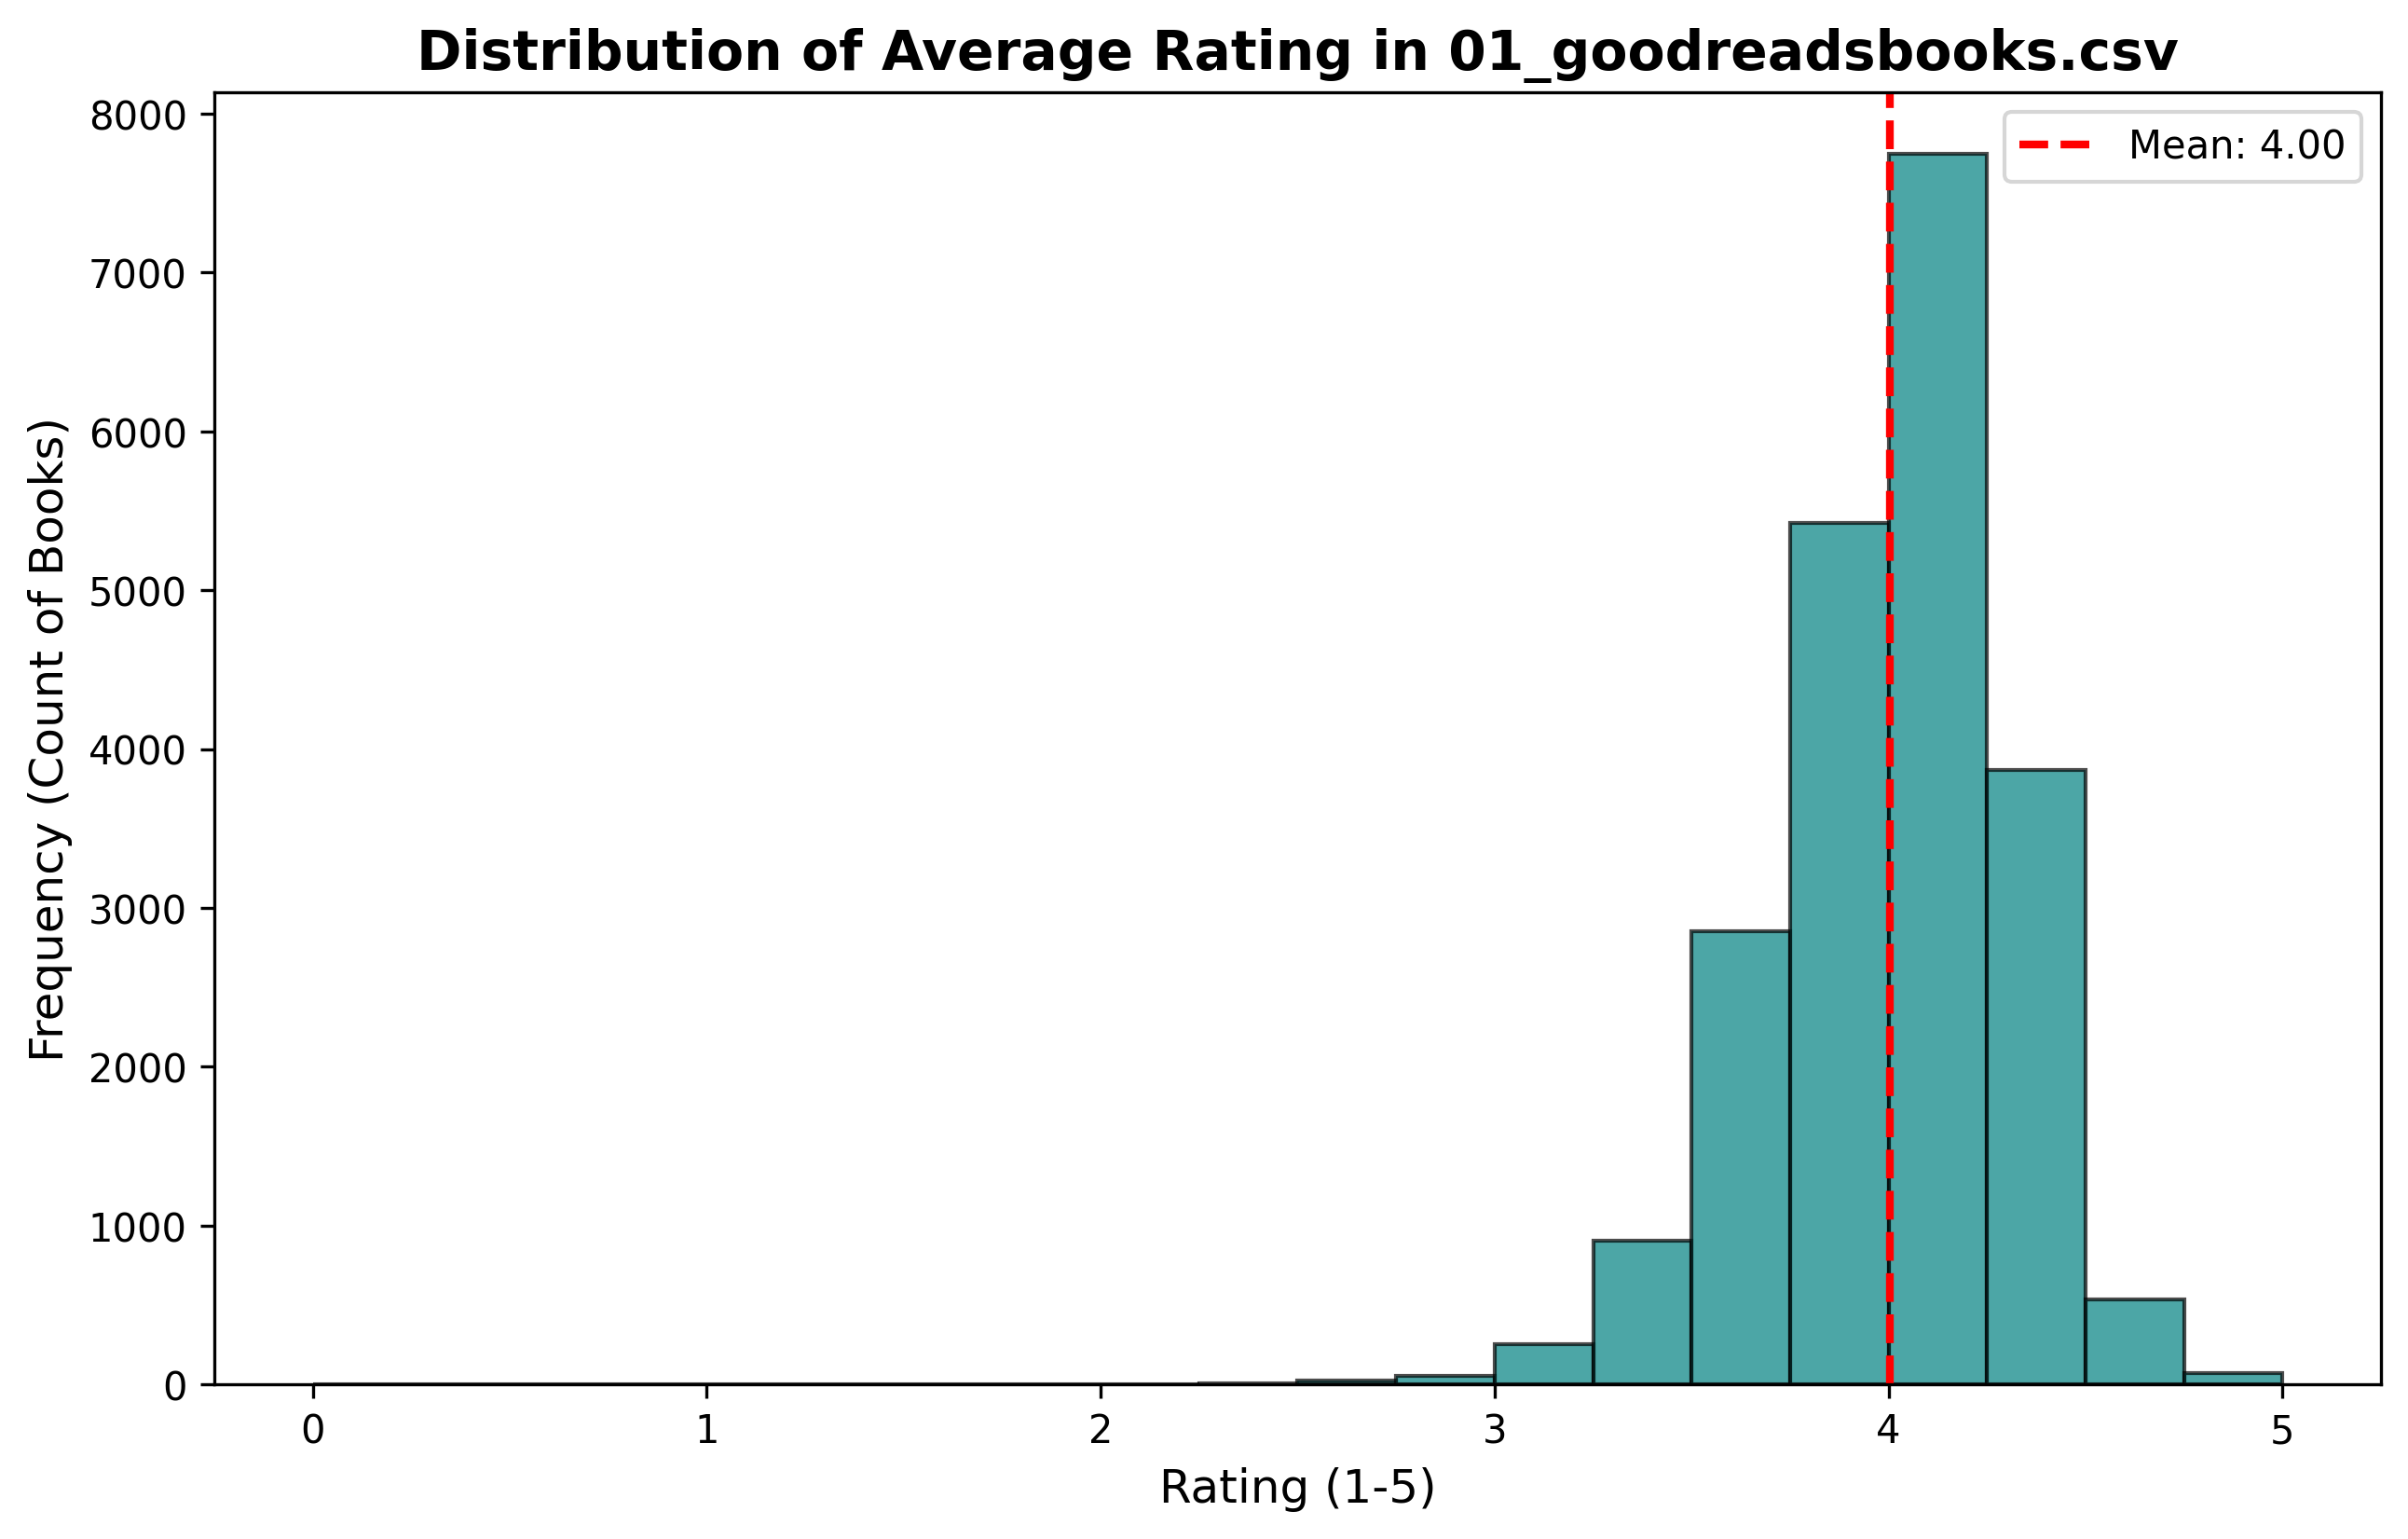
\includegraphics[width=0.8\linewidth]{rating_histogram.png}
    \caption{Distribution of books rating in 01\_goodreadsbooks.csv}
    \label{fig:placeholder}
\end{figure}

Examining the histogram of the average ratings of romance books in the 01\_goodreadsbooks.csv we find that most readers rated the books around 4. This suggests that romance readers find books great reads. They often are not critical of books.

\subsubsection{Shelf Tag Distribution}

Analysis of the raw \texttt{shelves\_list} indicated that administrative tags like `to-read' originally dominated the dataset. During the preprocessing phase, we implemented a filter to remove these generic administrative tags to ensure our algorithms would focus on actual book shelves.

As shown in Figure \ref{fig:tag_frequencies}, the most prevalent tags post-cleaning include massive macro-genres such as fiction, romance, and fantasy. Establishing this baseline distribution is critical, as it directly foreshadows our findings for Discovery Question 1, where our association rule mining revealed that the community heavily favors cross-tagging with these broad, overarching categories rather than niche sub-genres.

\begin{figure}[hbtp]
    \centering
    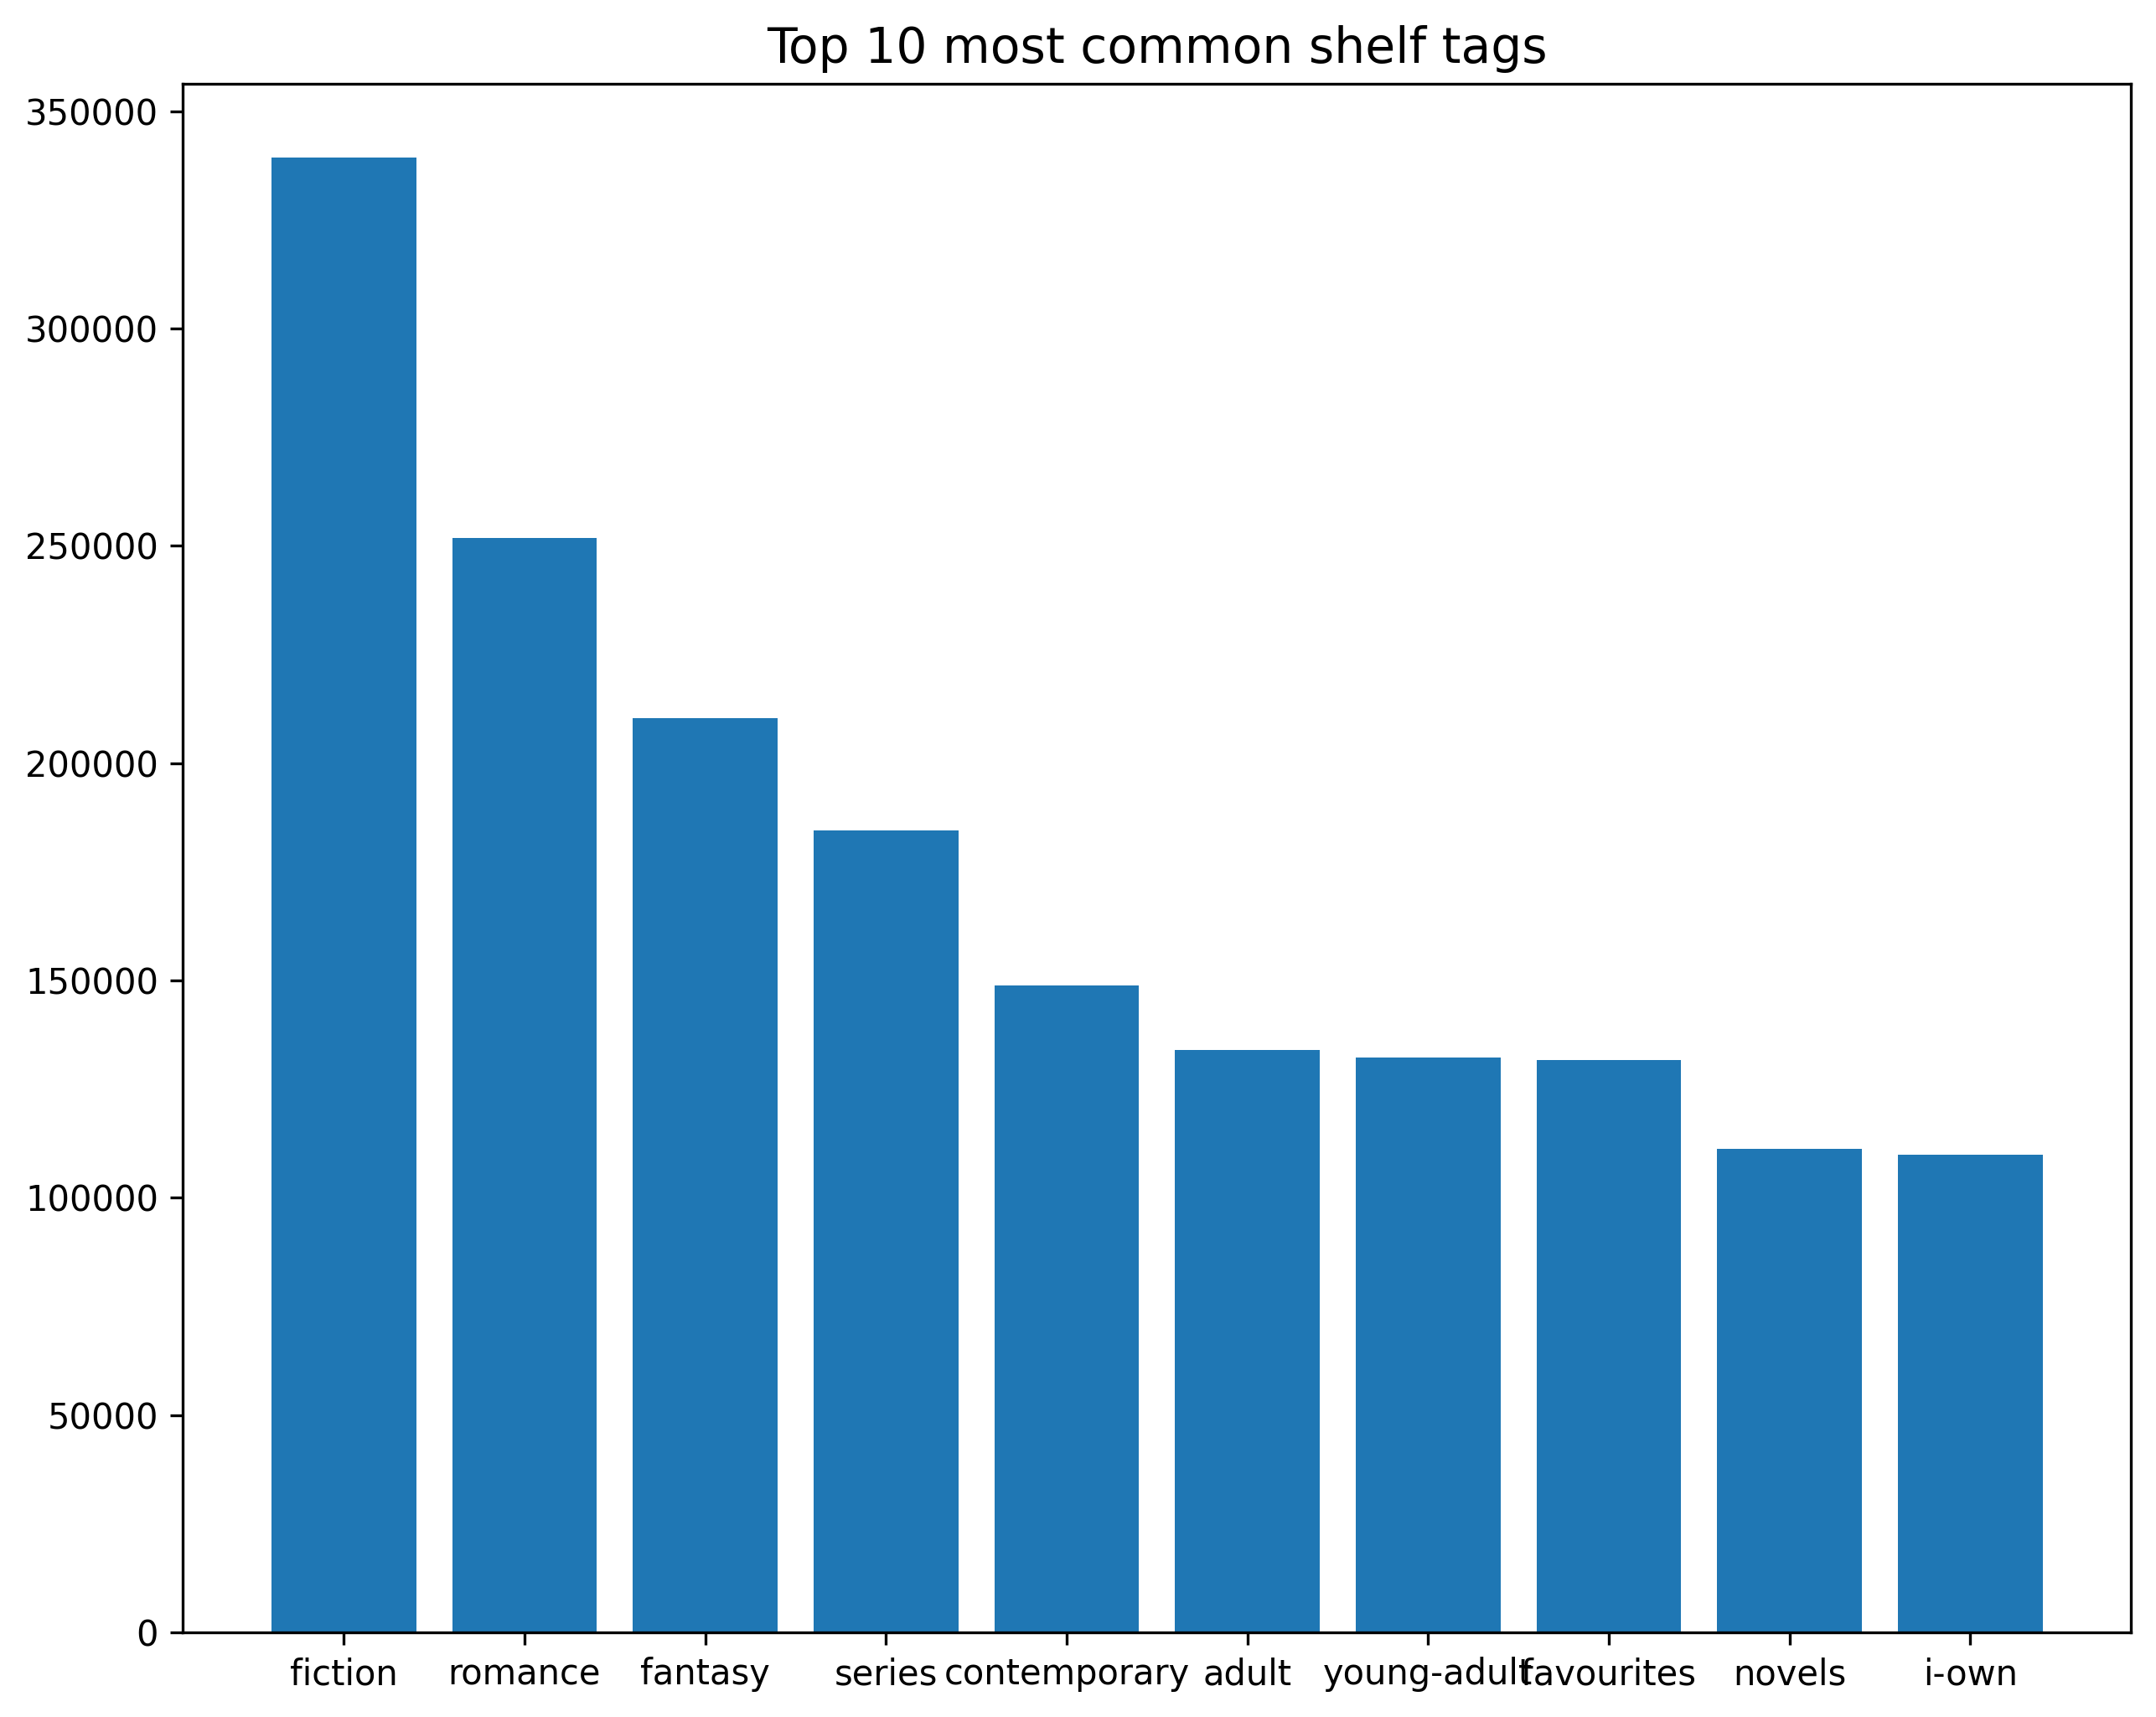
\includegraphics[width=\linewidth]{10commonbargraph.png}
    \caption{Distribution of the top 10 most frequent shelf tags post-cleaning}
    \label{fig:tag_frequencies}
\end{figure}



\subsection{Answering Discovery Question 1: Genre Associations}

Our team originally proposed if readers of ``Romantasy'' (Romance Fantasy) also showed high interest in other specific romance sub-genres. During our inital run developing our implementation for Milestone 2 our FP-Growth algorithm generated relationships based off structural administrative tags rather than genre relationships like romance. Furthermore, variations in user-generated text caused our target genre to be heavily diluted. To correct this for Milestone 3, we implemented a data normalization pipeline to aggregate variations of Romantasy (e.g., ``fantasy romance'', ``paranormal romance'') into standardized categories. We also significantly lowered our algorithm parameters, dropping the minimum support threshold to 0.01 (1\% of transactions) and the minimum lift threshold to 2, to ensure we were not filtering out niche sub-genre connections.


\begin{table}
\caption{Top Discovered Genre Association Rules (Min Support = 0.01)}
\label{tab:association_rules_m3}
\begin{tabular}{llcc}
\toprule
antecedents & consequents & lift & support \\
\midrule
{supernatural} & {vampire, paranormal-fantasy} & 7.520000 & 0.019000 \\
\bottomrule
\end{tabular}
\end{table}


Even with our highly sensitive thresholds and normalized data, the dataset did not support our inital hypothesis. The FP-Growth algorithm did not find any strong association rules linking 'Romantasy' or other related genres to other specific categories. This suggests that users who tag books with 'Romantasy' tend to treat it as a standalone category. Cross-tagging these books they tend to be associated with broad labels. This null result provides a clear answer to our first discovery question: Readers do not typically engage in sub-genre cross-pollination within the romance category. Instead, ``Romantasy'' serves as a descriptive tag for these users.

\begin{figure}[hbtp]
    \centering
    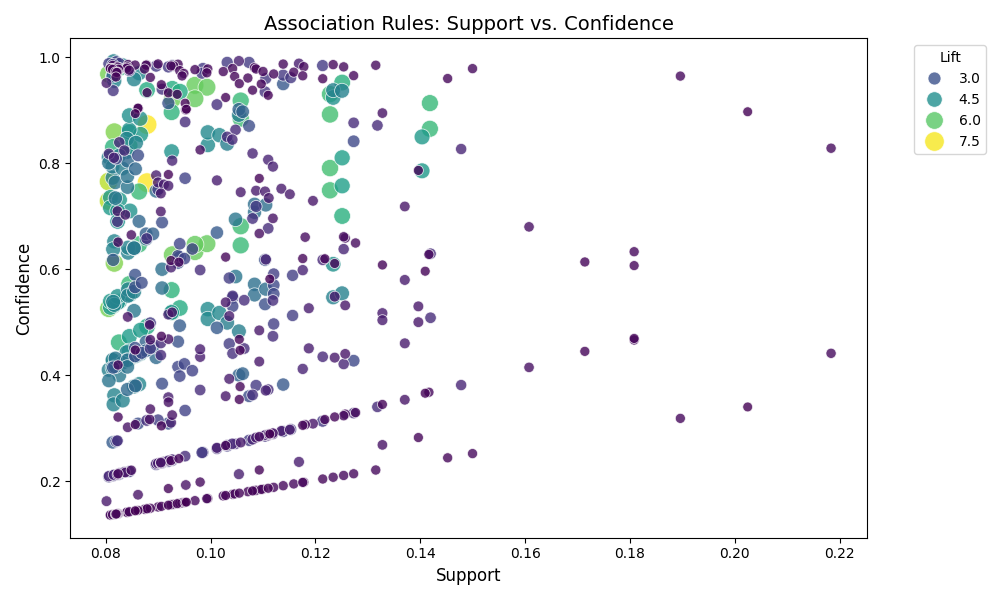
\includegraphics[width=\linewidth]{04_associationrules.png}
    \caption{Genre Associations}
    \label{fig:association_rules}
\end{figure}




\section{Milestone 3}

Moving into Milestone 3, our plan remains aligned with the original Milestone 1 proposal. Since we have successfully established our preprocessing pipeline and validated our association rules, our next focus will be applying K-Means clustering to answer our second discovery question. We will collect user interactions from rating variance and review length—to identify distinct reader categories (e.g., casual consumers vs. critical reviewers). Additionally, we will begin exploring Latent Dirichlet Allocation (LDA) for text mining the review bodies.

\subsection{Results/Pattern Discovery}

\subsection{Discovery Question 2: Reader Personas}

For the second discovery question our team asked if we could categorize users as a "critical reviewer" or a "casual consumer" based off average rating variance, review frequency, and review length. In order to measure these users, our team developed a K Means analysis using Elbow charts to create 4 clusters of users based off {review_frequency, avg_rating, rating_variance}.

Based on our K-Means clustering, we identified a "Casual consumer" in Cluster 1. These readers do not rate books very often or leave a lot of reviews. However they do tend to be very critical in their reviews as their average rating is only a a 2.94.

\subsection{Discovery Question 3: Engagement Volume}

Our team's final discovery question asked if patterns could emerged from highly up-voted reviews compared to reviews with a lot of down votes or no votes at all. A Pearson correlation analysis revealed a notable moderate positive correlation
Beyond genre tags and ratings, we extracted user engagement metrics from the \texttt{goodreads\_reviews\_dedup.json.gz} dataset to identify behavioral patterns. A Pearson correlation analysis reveals a notable moderate positive correlation of $0.52$ between the number of comments (\texttt{n\_comments}) and the number of votes (\texttt{n\_votes}), suggesting that reviews sparking discussion are also more likely to be perceived as helpful or popular. Conversely, our initial hypothesis that \texttt{review\_length} would drive higher engagement was unsupported, as it maintained negligible correlations with both \texttt{n\_votes} ($0.03$) and \texttt{n\_comments} ($0.04$). Furthermore, the numerical \texttt{rating} appears entirely decoupled from interaction volume, showing correlations of $0.00$ and $-0.01$ against votes and comments, respectively. These results indicate that while social interactions (voting and commenting) tend to scale together, they are driven by factors other than the sentiment of the rating or the verbosity of the review.

\begin{figure}[hbtp]
    \centering
    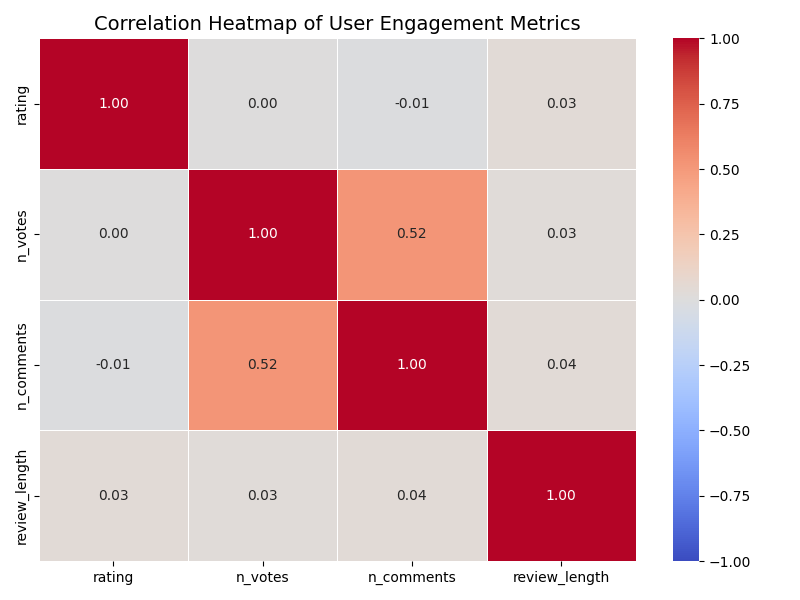
\includegraphics[width=0.8\linewidth]{correlation_heatmap.png}
    \caption{Correlation Heatmap of User Engagement Metrics}
    \label{fig:user_engagement}
\end{figure}

Visualizing this relationship via a scatterplot (Figure \ref{fig:engagement_scatter}) confirms the heatmap findings. While the majority of reviews cluster near the origin of the graph, there is a clear positive trend where reviews exceeding $1,000$ votes frequently receive over $150$ comments. These results indicate that while social interactions (voting and commenting) tend to scale together, they are driven by community relevance of a review rather than the sentiment of the rating or the content of a certain book.
\begin{figure}[hbtp]
    \centering
    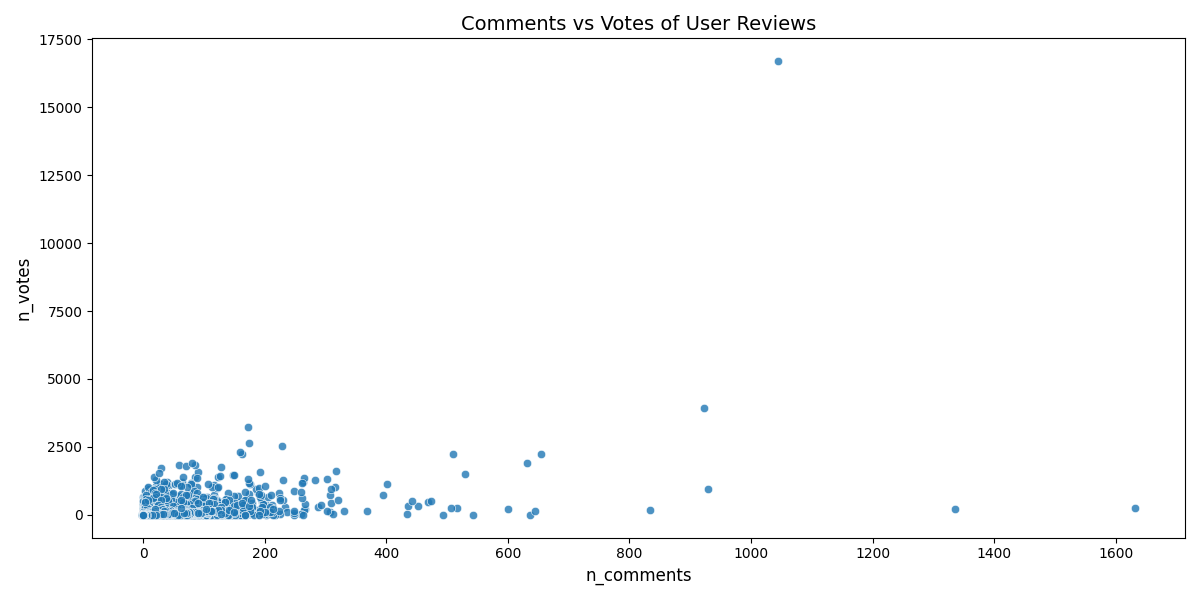
\includegraphics[width=0.8\linewidth]{scatterplot_commentvotes.png}
    \caption{Scatterplot of Comments vs. Votes}
    \label{fig:engagement_scatter}
\end{figure}



\section*{Acknowledgment}
The author would like to thank Julian McAuley for providing the Goodreads dataset and Kennesaw State University for the computational resources.

\begin{thebibliography}{00}
\bibitem{b1} Mengting Wan, Julian McAuley, "Item Recommendation on Monotonic Behavior Chains", in RecSys'18.
\bibitem{b2} Mengting Wan, Rishabh Misra, Ndapa Nakashole, Julian McAuley, "Fine-Grained Spoiler Detection from Large-Scale Review Corpora", in ACL'19

\end{thebibliography}

\end{document}
